\chapter*{Практика 3. Перемежение}
\addcontentsline{toc}{chapter}{Практика 3. Перемежение}
\label{ch:3_practice}

\textit{\textbf{Задание:}} Реализовать перемежитель для распределения пакетных ошибок.

\begin{itemize}
    \item Разработаны функции перемежения и деперемежения
    \item Реализовано сохранение индексов перемежения для корректного восстановления
    \item Добавлена проверка размерностей входных данных
    \item Проведено тестирование корректности работы
\end{itemize}

\begin{figure}[ht]
    \centering
    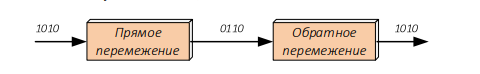
\includegraphics[width=0.8\textwidth]{interleaver_scheme.png}
    \caption{Структура перемежителя и деперемежителя}
    \label{fig:interleaver_scheme}
\end{figure}

\begin{figure}[ht]
    \centering
    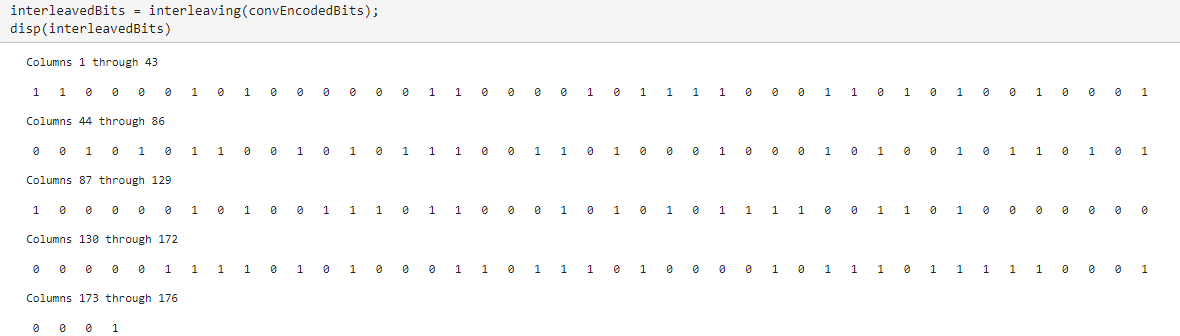
\includegraphics[width=0.8\textwidth]{3practice_result.png}
    \caption{Результат третьей практики}
    \label{fig:3practice_result}
\end{figure}